%!TEX root = ../BoYu-Dissertation.tex
\graphicspath{{Figures/}}

\chapter{A Design Framework for Awareness Promotion} % (fold)
\label{cha:design_framework}

Following the conceptual model of awareness phenomena in complex collaborative activities, we present a design framework for awareness promotion in this chapter. The framework describes the different means to promote awareness based on our conceptual framework, and is used to review existing awareness system designs, then lead to the rationale for our computational approach.

\section{A Review on Existing Computational Models} % (fold)
\label{sec:a_review_on_existing_computational_models}


Event notification model (GroupDesk, PoLIAwaC et al.)
Spatial model
Focus/Nimbus Model
Diffusion
Atmosphere

Dimensions
Field of Work: activity, local scope, dependencies
Processes: perception, interpretation, decision-making, action, propagation
Interplay: 
whether the filed of work can be updated by the processes
whether the processes are supported by explicit representation of field of work

% section a_review_on_existing_computational_models (end)

\section{Formalizing the Field of Work in SharedPlan Theory}
Rooted in the SharedPlans theory \cite{grosz1996collaborative,Grosz98theevolution}, the proposed activity model treats a collaborative activity as an evolving shared plan situated in a set of physical and mental contextual factors. In general, a shared plan is a moment-to-moment representation of an unfolding activity and includes not only a hierarchy of actions but also the set of mental states (beliefs, intentions, and commitments) that the participating actor have established towards the activity, and the knowledge preconditions and physical constraints that have to be satisfied prior to an activity being performed.

\subsection {SharedPlan Theory}
\subsubsection*{Action Decomposition}
The SharedPlans theory models an activity as hierarchically structured subsidiary actions that are intended and performed in some specific context components. An \textbf{action} refers to a specific goal as well as the effort needed to achieve it. An action can be either basic or complex. A \emph{basic} action can be directly executed by one or multiple actors. A \emph{complex} action, however, cannot be directly executable because it needs to be decomposed into subsidiary actions. The concept of action in SharedPlan theory has a broad definition, which includes the high-level collaborative activity, the medium-level actions, and the low-level operations.

The knowledge preconditions are called \textbf{parameters} of the action that have to be identified prior to an action being performed, i.e. actors must be able to identify the parameters of the action to be performed. A parameter can represent the knowledge about an object of the action or a resource used by the action. It is shared and visible to the action it belongs to and all the sub-actions. If a parameter has not been identified, the actors need to develop a plan to identify the parameter before the action can be performed.

A \textbf{precondition} defines a certain proposition that indicates certain states of a parameter or relationships among multiple parameters must be satisfied in order to perform an action. As a result, any variables in a precondition must also appear in the action's parameter list. 

\subsubsection*{Mental States}
The SharedPlans theory provides a formal specification of the mental attitudes requirements of participants in a collaborative activity. The specification is given in terms of beliefs, mutual beliefs, and intentions of the participants. It deploys two intentional attitudes, intending to (do an action) and intending that (a proposition hold). Intentions-to are used to represent an agent’s commitments to its own actions. Such commitments instigate means-end reasoning about ways of accomplishing its intended actions – that is, to planning. Intentions-that are used to represent an agent’s commitments toward a joint activity and the actions of its fellow participants in service of that activity. Such commitments lead an agent to engage in reasoning about other participant’s actions and intentions and ways the agent could contribute to their success in the context of the group activity. Besides, an indicator of the current attentional state, representing whether an action is the current focus of an actor is also included. 

\subsubsection*{Partiality of Plans}
A critical point made in the SharedPlans theory is that planning is interleaved with acting, which means agents can act on partial recipes, and a group of agents may not have a complete plan until after they have done some of the actions in the partial recipe. To have a partial shared plan means there are still some actions that remain to be resolved (i.e., role assignment) or decomposed further. In the beginning of the collaboration, the agents only have a partial shared plan of the activity, which merely consists of the agent’s initial intention of performing the activity. With the development of the activity, the agents collaboratively elaborate the activity by selecting recipe for it, breaking it down into subsidiary actions, and updating their beliefs and intentions towards these subsidiary actions. In this course, the shared plan evolves and when it reaches the status of a full shared plan, the collaboration ends up with the underlying activity successfully performed.

The SharedPlans theory has the benefits to address the aforementioned challenges of modeling an activity:  (1) the internal mental states of the user are modeled as the intentions, beliefs, and mutual beliefs of the participants; (2) the activity is modeled as hierarchically structured actions that are intended and performed in some specific context components (e.g. constrains, knowledge preconditions, intentional structure, and attentional state etc.); (3) the development of an activity is modeled as the evolution from a partial shared plan to a full one. 

A plan of an action is a description of the action in the specific collaborative context. The difference between a plan and a recipe of an action can be drawn from two aspects: first, a plan indicates the specific way to perform the action, which is generated in the collaborative activity. It can be considered as the internal representation of the underlying activity. But a recipe represents the external knowledge about how to perform an action. Second, a plan includes the mental states of the agents towards the action. The major components of mental states for a plan include: (1) Intentions. Based on SharedPlan theory, we distinguish between two kinds of intentions: intentions to perform an action (IntTo) and intentions that a proposition holds (IntThat). An agent intending to do an action must commit to doing that action, and must hold appropriate beliefs about its ability to perform the action. IntThat is used to represent an agentÕs expectation that some proposition will hold or some actions will be performed (possibly by other agents). An agent intending that a proposition holds must be committed to doing what it can to help make the proposition hold. (2) Beliefs refer to what human agents believe about the action. They can be beliefs about the completion of the action, the value of a parameter, the way to perform the action, or the ability of the agents to perform the action.

\subsection{Activities} % (fold)
\label{sub:activities}

% subsection activities (end)

\subsection{Local Scopes} % (fold)
\label{sub:local_scopes}

% subsection local_scopes (end)

\subsection{Dependencies} % (fold)
\label{sub:dependencies}

% subsection dependencies (end)

% section representing_knowledge_with_plangraph_model (end)

\section{Event-Driven Awareness Process}
\label{sec:event_driven_awareness_process}

\subsection{Events: the basic unit of awareness information} % (fold)
\label{sub:understanding_events}
The application of event-based model offers high potential for awareness support in geo-collaboration. As we described in Chapter 1, many geo-collaborative work settings are characterized by different types of dynamics, such as when cooperation breaks down, changes over time, and is perceived differently by different actors involved. Understanding the dynamics of cooperative work is extremely important as a way to understand how to design computer systems supporting coordination. If computer technology does not take into account support for the dynamic development, change, and breakdown in cooperation, the system fails \cite{bardram1998designing}. As a result, we consider managing the contingencies inherent to coordination work, and assume that coordination work always become necessary when certain state of the collaborative work changes, or the normal flow of work breaks down. It is the state changes in the field of coordination work that cause the actors to identify changing dependency relations, and try to resolve possible problems or conflicts \cite{symon1996coordination}. Following this argumentation, we believe that events offer a unifying and powerful abstraction to describe the necessary awareness information needed for coordination in geo-collaboration. 

\subsubsection{The concept of events} % (fold)
\label{ssub:the_concept_of_events}
The concept of events has been used in the literature from different perspectives \cite{worboys2005a}. In general, we can distinguish two different classes: \emph{ontological} and \emph{cognitive} positions. 

In the \emph{ontological} position, set out by Quine \cite{quine1985events}, events and objects are not to be distinguished, as both are first-class entities that can be localized in space and time, broken into sub-parts, and arranged in a taxonomic hierarchy. Events are defined as the occurrences in the real world and \emph{the goal of modeling the events primarily focuses on study the internal structures of the events}. For example, a traffic accident can be considered as an instance of an event type \emph{TrafficIncident}. Event types can be arranged in a subsumption hierarchy; for example, event type \emph{TrafficIncident} may subsume \emph{SeriousTrafficAccident}. Events may have parts; for example, \emph{SeriousTrafficAccident} may be composed of an event of \emph{AccidentReport} and an event of \emph{EmergencyResponse} \cite{worboys2005a}.  

On the other hand, the \emph{cognitive} perspective defines an event as a linguistic or cognitive concept that supports the interpretation of a significant pattern of change \cite{allen1994actions}. That is, the world does not really contain events. Rather, events are the way by which agents classify certain useful and relevant patterns of change. The very same circumstance in the world might be described by any number of events. Each of these descriptions is a different way of describing the circumstances. No one description is more correct than the other, although some may be more informative for certain circumstances, in that they help predict some required information, or suggest a way of reacting to the circumstances \cite{allen1994actions}.\emph{Rather than studying the internal structure of events, modeling events from the cognitive position has mainly concentrated on what external inferences can be made from the fact that certain events are known to have occurred.} The event indicating the occurrence of a traffic accident is used to analyze possible impacts on the agent's work. For instance, the traffic accident may block the traffic flow, which make the agent's task of delivering an equipment to a destination difficult to finish on time. 

In the literature of GIScience, models of geographical events have been proposed to study the dynamic geographic phenomena \cite{worboys2005a}. The concept of events in these models usually belongs to the ontological position. For example, in \cite{YuanApril20011523-0406-83}, complex geographical phenomena,such as wildfire or precipitation, have been modeled in a hierarchy of events, processes, and states. The purpose is to study the internal structure of an event. In the case of precipitation, an event marks the occurrence of precipitation in a study area. A process describes how it rains; that is the transition of precipitation states in space and time. In \cite{rodriguez2005a}, the object-oriented approach has been adopted to model all the types of occurrences in a habor's zones. The focus here is to derive the different event types that may occur in a habor and identify the relationships between them.   

In the context of awareness systems, however, events are mostly defined from the cognitive position. A common theme is that events are defined as changes that exemplify a property or relationship in some locations or objects at some time. It is an application-driven concept. A specific class of events usually defines a specific type of awareness information that is supported by an awareness system. For instance, the AREA system \cite{fuchs1999a} describes events as actions performed on an artifact and the event classes are derived from the artifact class hierarchy and possible operations on them. The ENI system \cite{gross2004a} describes events from the sensors associated with actors, shared artifacts, or any other objects that generate events related to them. The primitive events represent low-level change units obtainable from individual sensor data streams. Composite events are aggregates of primitive events from single or multiple sensor data streams. An event is represented as an attribute-value tuple that represents an instance of an event type that is supported by an awareness system.
% subsubsection the_concept_of_events (end)

\subsubsection{Why Event-Driven?} % (fold)
\label{ssub:why_event_driven_}

1. unstable communication link

2. information push v.s. pull

3. dynamics in activities

% subsubsection why_event_driven_ (end)

% subsection understanding_events (end)
\subsection{Event-driven awareness process} % (fold)
\label{sub:event_driven_awareness_process}

By distinguish different types of events, the proposed awareness mechanism follows the event processing architecture (Taylor et al., 2009), and is performed in following steps: 

(1) \emph{Event generation}. Sensors recognize external events, which are represented as event objects within the system. 

(2) \emph{Event interpretation}. Event interpretation components/actors evaluate direct implications of these external events on their activities, and derive new internal events. 

(3) \emph{Event propagation}. Event propagation components/agents reason on top of these initial state changes to understand their chain effects on other activities through the web of dependency relationships. 

(4) \emph{Event notification}. All the relevant local and derived remote events are notified to the users based on their subscriptions within their local scope of interests 

Figure \ref{fig:event_process} illustrates an example of how these steps are performed to process a single event, and how the knowledge about the field of coordination work (activities, local scopes, and dependencies) are used in the awareness process. This awareness process starts with the detection of an external event by a sensor. During the interpretation phase, the knowledge about current states of activities and their dependencies is employed as the inferential framework to understand the state changes revealed by the event, and update the current states of these components within the collaborative activity, which generates a new internal event. Due to the existence of the web of dependencies among activities, the initial internal event can (or potentially can) lead to changes outside the original actor’s local scope of work. The inference of effects on other remote activities is performed during the propagation step, and a list of derived internal events can be generated. If any of the events is defined within an actor's local scope of work, the actor will be notified about the change during the notification step.

Figure. 1 demonstrates how the awareness process works on top of the three constructs. In the beginning, Actor 1 perceives some unexpected event happening in the environment, and attempts to interpret it as whether and how it can impact the activities within her local scope of work. After understanding the event, she associates it with a state change of Activity 1. Furthermore, she predicts how the state change of this activity will impact other activities because of the dependencies among them. After Actor 1’s projection, the event is likely to impact another activity (Activity 2), which also falls into Actor 2’s local scope of work. Upon receiving this projection from Actor 1, Actor 2 first needs to understand where this projected event comes from by backtracking the interpretation, and evaluate how this event will impact his own line of work, which leads to a new projected state change of Activity 3. The similar process then is propagated to Actor 3’s local scope of work. In this way, the team’s awareness of the initial external event is collaborative developed as the relevant actors gradually attach their interpretations to it.

\begin{figure}[htbp] %  figure placement: here, top, bottom, or page
   \centering
   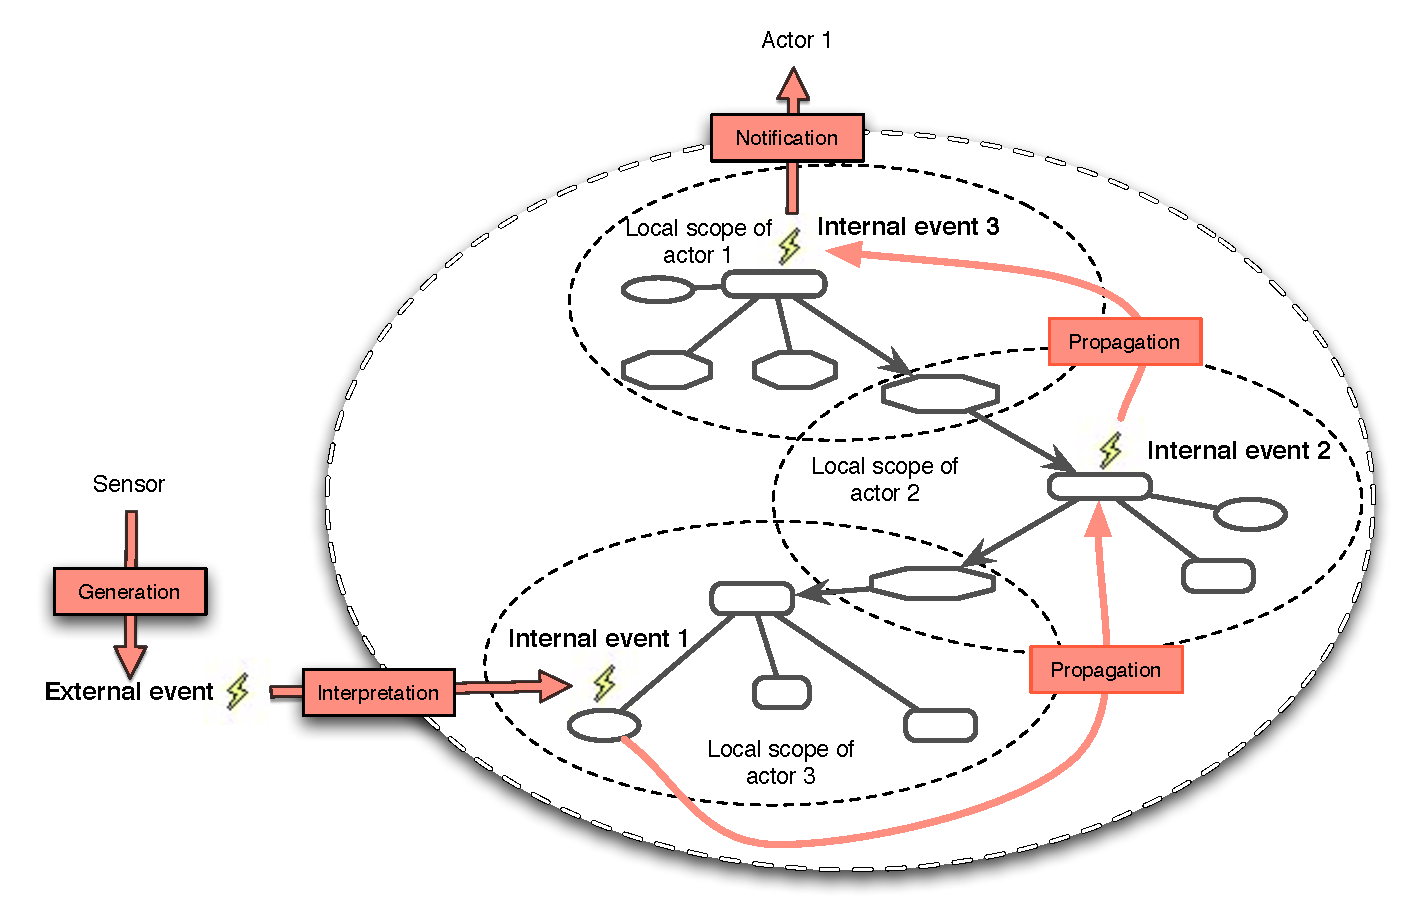
\includegraphics[width=5.5in]{event_process.pdf} 
   \caption{Event-based awareness process}
   \label{fig:event_process}
\end{figure}
% subsection event_driven_awareness_process (end)
% section event_driven_awareness_process (end)

\section{Mediation Roles of the Computer} % (fold)
\label{sec:mediation_roles_of_the_computer}

Our design for computer-supported awareness promotion focuses on the mediation roles that the system can play to support awareness development. 

\begin{enumerate}
	\item It provides the visual and interactive support that allow the users to interpret awareness information within their local scope of work. As the awareness information is propagated across multiple actors, the chain of reasoning can become very lengthy. By visualizing the event propagation chains with context information about activities, the users can backtrack how the awareness information is developed from the origins.
	
	\item It supports the relay of awareness information across local scopes. Although the actors have best knowledge within their local scopes of work to interpret and develop awareness information,  they often do not know who will be interested in receiving their interpretations. By maitaining a computational model of the ongoing activities and local scopes, the system can recognize whenever the interpretation transcends the boundaries of multiple local scopes and relay the awareness informaton to other actors.
	
	\item With the situated knowledge about activities and their dependencies, the system can play a even more proactive role to automate the reasoning on how certain awareness information impact the states of activities as its effects propagate across multiple activities. In this way, the system can offload some of the interpretation effort from the human actors. Meanwhile, the human actors should have the capability to revise the system’s interpretation.
	
\end{enumerate}

In this study, we operationize these mediation roles within an event notification system to promote awareness. We consider events as basic units of awareness information, representing changes concerning the environment, resources, goals, and activities in a collaborative setting. We make distinctions between external (in the environment) and internal events (in the activities). External events are changes in the physical environment that have impact on the performance of activities. Internal events are state changes on any resources, goals, and activities involved in the collaboration.

By adopting the event-driven approach, the mediation roles of the system to support transitive awareness process can be illustrated in Figure \ref{fig:comp_framework}. Whenever an external event is sensed by the system, it first matches the events with all the users’ predefined local scope of work and their subscriptions. If a match is found, the system notified the matched user (e.g. Actor 1) about the external event. Then upon perceiving the event, Actor 1 interprets the direct impacts of this event on his/her current activities and predicts future changes to other activities within his/her local scope of work. The inferred state changes represented as internal events are then sent back to the system. The system reasons about how these predicted changes by Actor 1 may impact other actors due to the dependencies among activities, and notify the projected state changes to other relevant users (e.g. Actor 2). Upon receiving the notification about the projected state change, Actor 2 needs to interpret the change by backtracking where this state change comes from and relating it to the activities within his/her local scope of work. Actor 2 may reject the system inference by revising the belief about the projected state change, or predict further changes due to this change, which leads to a new cycle of reasoning.

\begin{figure}[htbp] %  figure placement: here, top, bottom, or page
   \centering
   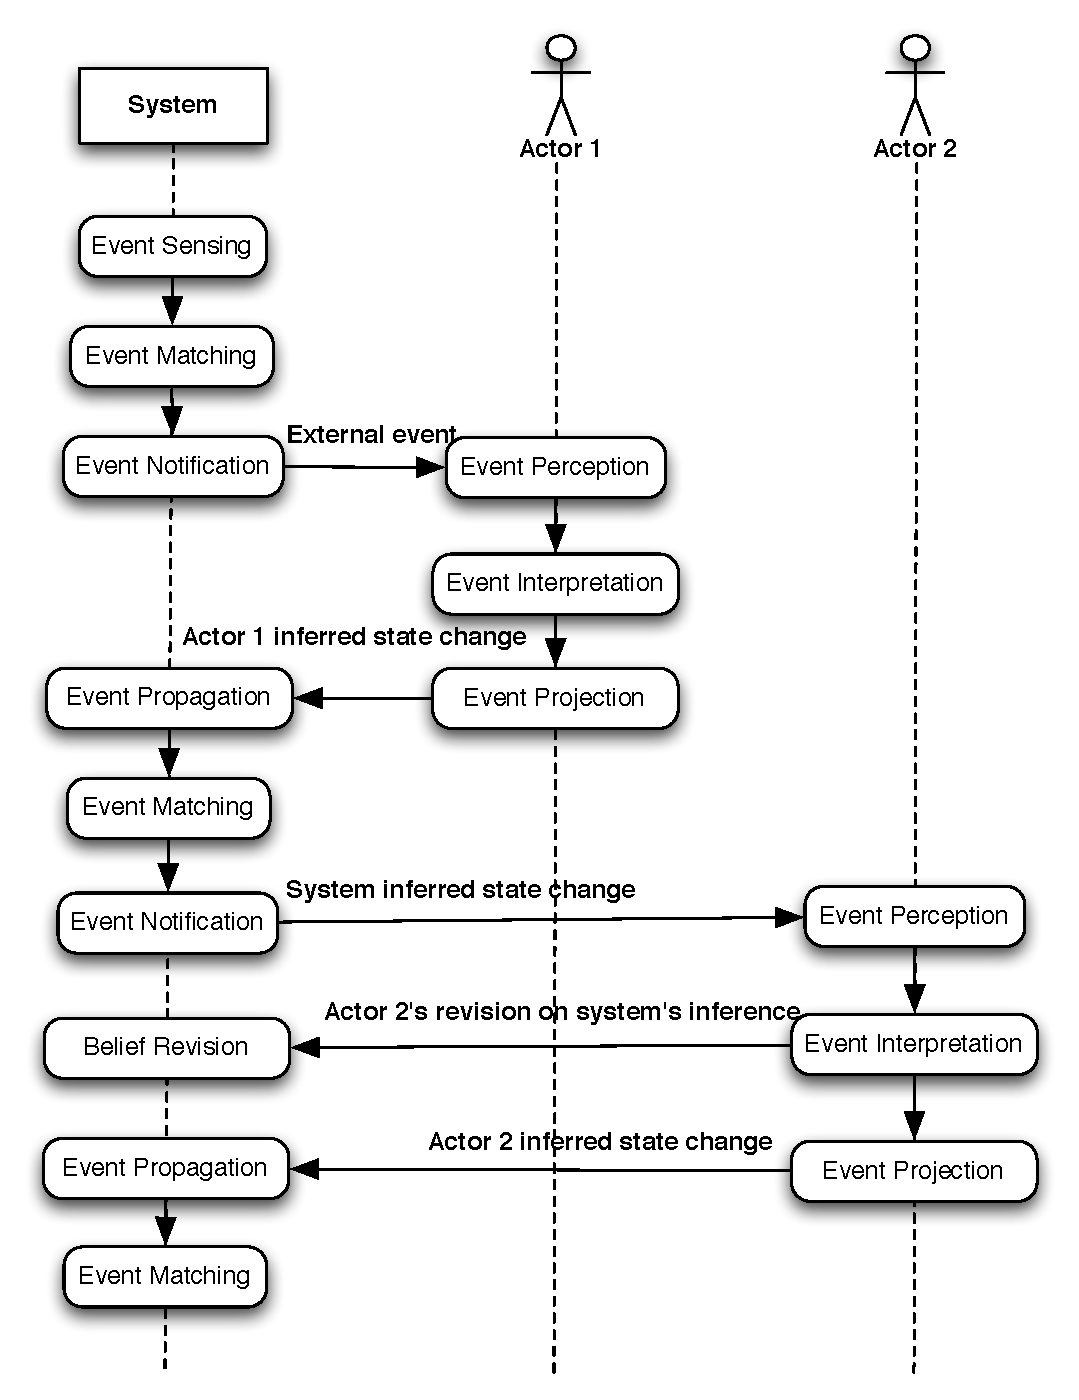
\includegraphics[width=5.5in]{comp_framework.pdf} 
   \caption{Event-based awareness process}
   \label{fig:comp_framework}
\end{figure}
% section mediation_roles_of_the_computer (end)


% chapter design_framework (end)




 

